\chapter{Convolution of Piecewise Functions}

Convolution is an operation which takes two functions and produces a third.
It takes one of the two input functions, and modifies one by mirroring and translating.
The resulting function is then the overlap between one of these functions as a function of the translation.
Visually, this can be seen below in Figure~\ref{fig:ConvolutionExample}.

\begin{figure}[ht]
	\caption[Convolution of box signal with itself]{The convolution of the box signal 
	$f(t)=g(t)=\left( 0^\oiOpOp{-\infty,-0.5} \oplus 1^\oiClCl{-0.5,0.5} \oplus 0^\oiOpOp{0.5,\infty} \right)$ with itself.
	\label{fig:ConvolutionExample}}
	\centering
	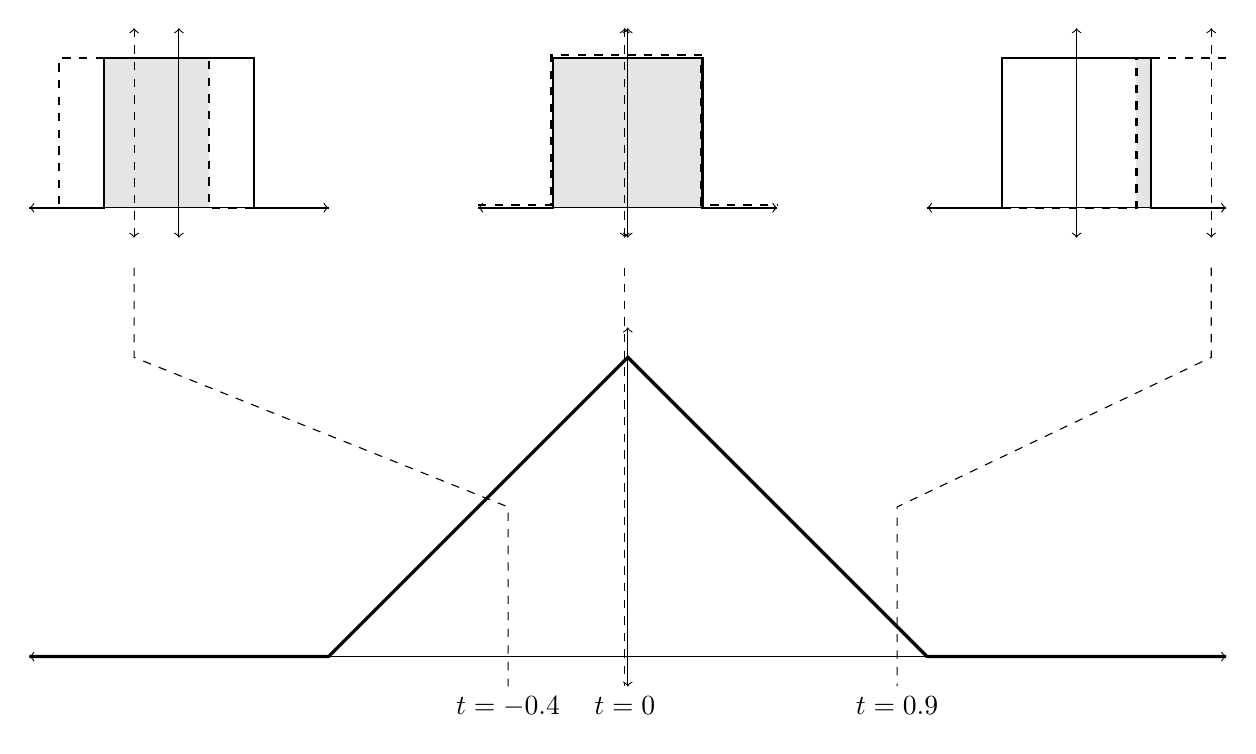
\begin{tikzpicture}[scale=3.8]
		\draw[fill, color=black!10] (-1.75,1.5) rectangle (-1.4,2);	
		\draw[fill, color=black!10] (-0.25,1.5) rectangle (0.25,2);	
		\draw[fill, color=black!10] (1.75,1.5) rectangle (1.7,2);	
	
		\draw[<->] (-2,0) -- (2,0);
		\draw[<->] (0,-.1) -- (0,1.1);
		\draw[very thick] (-2,0) -- (-1,0) -- (0,1) -- (1,0) -- (2,0);
			
			
		\draw[<->] (-2,1.5) -- (-1,1.5);
		\draw[<->] (-1.5,1.4) -- (-1.5, 2.1);
		\draw[dashed, <->] (-1.65,1.4) -- (-1.65, 2.1);
		
		\draw[<->] (-.5,1.5) -- (.5,1.5);
		\draw[<->] (0,1.4) -- (0, 2.1);
		\draw[dashed, <->] (-0.01,1.4) -- (-0.01, 2.1);
		
		\draw[<->] (1,1.5) -- (2,1.5);
		\draw[<->] (1.5,1.4) -- (1.5, 2.1);
		\draw[dashed, <->] (1.95,1.4) -- (1.95, 2.1);
		
		
		\draw[thick] (-2,1.5) -- (-1.75,1.5) -- (-1.75,2) -- (-1.25,2) -- (-1.25,1.5) -- (-1,1.5);
		\draw[thick,dashed] (-2,1.5) -- (-1.9,1.5) -- (-1.9,2) -- (-1.4,2) -- (-1.4,1.5) -- (-1,1.5);
		
		\draw[thick] (-.5,1.5) -- (-.25,1.5) -- (-.25,2) -- (.25,2) -- (.25,1.5) -- (.5,1.5);
		\draw[thick,dashed] (-.5,1.51) -- (-.255,1.51) -- (-.255,2.01) -- (.245,2.01) -- (.245,1.51) -- (.5,1.51);
		
		\draw[thick] (2,1.5) -- (1.75,1.5) -- (1.75,2) -- (1.25,2) -- (1.25,1.5) -- (1,1.5);
		\draw[thick,dashed] (2,2) -- (1.7,2) -- (1.7,1.5) -- (1,1.5);


		\draw[dashed] (-0.01,1.3) -- (-0.01,-.1) node [below] {$t=0$};
		\draw[dashed] (-1.65,1.3) -- (-1.65, 1) -- (-0.4, 0.5) -- (-0.4,-.1) node [below] {$t=-0.4$};
		\draw[dashed] (1.95,1.3) -- (1.95, 1) -- (0.9,0.5) -- (0.9,-.1) node [below] {$t=0.9$};
		
	\end{tikzpicture}
\end{figure}

Formally this, equates to the following definition for convolution over continuous domains:
\begin{definition}
	The \textbf{convolution} $*$, of two functions $F$ and $G$ is defined as:
	\begin{equation}
		(F*G)(t) = \int_{-\infty}^\infty F(\tau) \;G(t - \tau) \; d\tau
	\end{equation}
\end{definition}
and in the case of discrete linear convolution, summation would replace integration.
In this equation, $t$ represents the translation of $G$ as well as the input for $(F*G)$
while $\tau$ is internal to the integral and varies over the real line.


\begin{figure}[ht]
	\caption[Gaussian Blurring]{512x512px ``Lena''(a) with a 1px (b) and 5px (c) Gaussian blur applied. 
	Gaussian blurring is accomplished by convolving an image with a Gaussian kernel and is commonly used
	in image processing to reduce noise prior to edge detection.
	\label{fig:LenaBlur}}
	\centering
	\begin{subfigure}[b]{0.3\textwidth}
                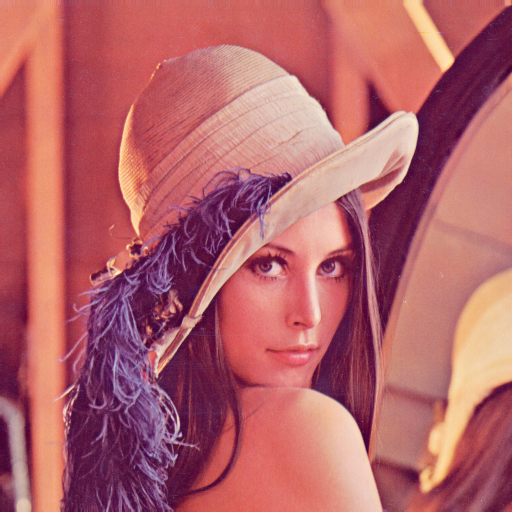
\includegraphics[scale=0.25]{diagrams/Lenna}
                \caption{Original Image}
       \end{subfigure}
       \begin{subfigure}[b]{0.3\textwidth}
                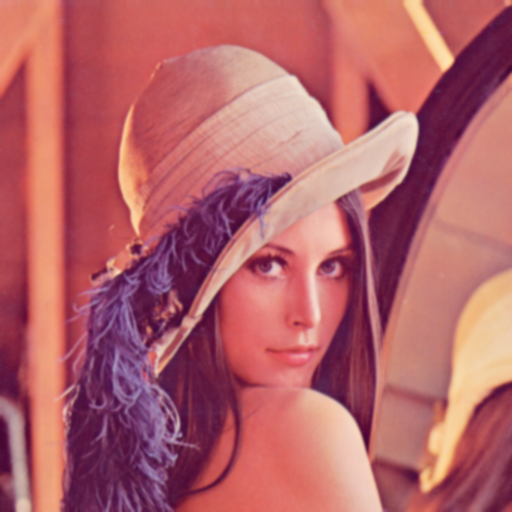
\includegraphics[scale=0.25]{diagrams/Lenna-blur1}
                \caption{1px Gaussian blur}
       \end{subfigure}
       \begin{subfigure}[b]{0.3\textwidth}
                
\includegraphics[scale=0.25]{diagrams/Lenna-blur5}
                \caption{5px Gaussian blur}
       \end{subfigure}
\end{figure}


Convolution has applications in many areas of mathematics and engineering.
One very common use in image processing is in blurring.
\emph{Gaussian blurring} is the result of a convolution in 2-dimensions of an image with the Gaussian distribution function:
\begin{equation}
	\label{eqn:2dGaussian}
	G(x,y) = \frac{1}{2 \pi \sigma^2} \; \text{exp} \left( - \frac{x^2 + y^2}{2\sigma^2} \right)
\end{equation}
Blurring an image in this way reduces noise and greatly increases the efficacy of subsequent edge detection.
In statistics, a (simple) \emph{moving average} can be represented as a convolution by a rectangular pulse while more
generally, weighted moving averages can be made by convolving with other functions.





%%%%%%%%%%%%%%%%%%%%%%%%%%%%%%%%%%%%%%%%%
%
% CONVOLUTION OF PIECEWISE
%
%%%%%%%%%%%%%%%%%%%%%%%%%%%%%%%%%%%%%%%%%
\section{Convolution of Piecewise Functions}\label{sec:PWConvolution}


CAS such as Maple and Mathematica are quite adept at solving integrals.
Convolution of elementary functions generally poses no problem.
When convolving two piecewise continuous functions, many possible intervals arise and the conditionals that arise
can quickly overwhelm them unaided.


We are interested in \emph{Symbolic Linear Convolution} (of piecewise continuous functions).
The typical approach is to first consider for convolution of ``one piece'' functions 
\cite{evans1994algorithms, west1993symbolic}.
By ``one-piece'' functions we mean functions which are restricted to a single interval and zero everywhere else.
We will consider two functions, $F$ and $G$ defined as:


\begin{equation}
	\label{eqn:fOnePiece}
	F(x)=f^{[a_f,b_f)}(x) = 
		\begin{cases}
			f(x) & a_f \leq x < b_f \\
			0 & \text{otherwise}
		\end{cases}
\end{equation}
\begin{equation}
	\label{eqn:gOnePiece}
	G(x)=g^{[a_g,b_g)}(x) = 
		\begin{cases}
			g(x) & a_g \leq x < b_g \\
			0 & \text{otherwise}
		\end{cases}
\end{equation}
for which we would like to compute the convolution $(F*G)$.
To reduce the total number of cases generated, it is generally also assumed that $b_f - a_f \leq b_g - a_g$.
Assuming that $F$ is non-zero over a shorter interval is not that strong an assumption as convolution is commutative;
if it is not the case we can rearrange $F*G$ to $G*F$.
To see this, simply apply the substitute $\tau' = t-\tau$ in equation (7.1):
\begin{align}
	\label{eqn:ConvCommutative}
	(F*G)(t) 
		&= \int_{-\infty}^\infty F(\tau) G(t-\tau) \;d \tau 
		\notag\\&= \int_{\infty}^{-\infty} F(t-\tau')G(\tau')\; (-1) d\tau' 
		\notag\\&= \int_{-\infty}^\infty G(\tau') F(t-\tau') \; d\tau'
		\notag\\&= (G*F)(t)
\end{align}


Thus we can assume that our static function is also the function with the shorter interval.
Since $F$ and $G$ are zero outside of their respective intervals, we do not need to integrate over the entire real line. 
$F$ is our static function, so $[a_f, b_f)$ would be sufficient.
For a tight boundary, we have the following:
\begin{align}
	\label{eqn:ConvNaiveOnePiece}
	(F*G)(t) 
	&= \int_{-\infty}^\infty F(\tau)\; G(t-\tau) \; d\tau \notag \\
	&= \int_{a_f}^{b_f} f(\tau) \; G(t-\tau) \; d\tau \notag \\
	&= 	\begin{cases}
			\int_{a_f}^{t-a_g} f(\tau) \; g(t-\tau) \; d\tau 	& (a_f+a_g) \leq t < (b_f+a_g) \\
			\int_{a_f}^{b_f} f(\tau) \; g(t-\tau) \; d\tau		& (b_f+a_g) \leq t < (a_f+b_g) \\
			\int_{t-b_g}^{b_f} f(\tau) \; g(t-\tau) \; d\tau	& (a_f+b_g) \leq t < (b_f+b_g) \\
			0										& \text{otherwise}
		\end{cases}
\end{align}


\begin{figure}[ht]
	\caption[Convolution of ``one-piece'' functions]{Convolution of length 1 and 2 rectangular pulses. 
	Given the functions $F=1^{[-1,1)}$ and $G=1^{[-2,2)}$, there are three non-zero regions in $(F*G)$.
	\label{fig:OnePiece}}
	\centering
	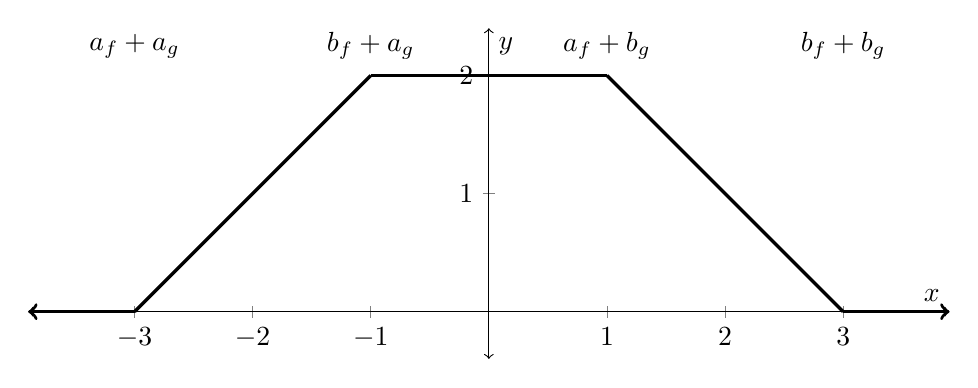
\begin{tikzpicture}
		\begin{axis}[
			x=1.5cm,
			y=1.5cm,
			xstep=1,
			ystep=1,
			xmin=-3.9,xmax=3.9,
			ymin=-0.4,ymax=2.4,
			axis x line=middle,
			axis y line=middle,
			axis line style=<->,
			xlabel={$x$},
			ylabel={$y$},
	        ]
		\addplot[no marks,black,very thick,<-] expression[domain=-3.9:-3,samples=100]{0};
		\addplot[no marks,black,very thick,-] expression[domain=-1:1,samples=100]{2};
		\addplot[no marks,black,very thick,-] expression[domain=-3:-1,samples=100]{x+3};
		\addplot[no marks,black,very thick,-] expression[domain=1:3,samples=100]{3-x};
		\addplot[no marks,black,very thick,->] expression[domain=3:3.9,samples=100]{0};
		\node(afag) at (axis cs:-3,2.25) {$a_f+a_g$};
		\node(bfag) at (axis cs:-1,2.25) {$b_f+a_g$};
		\node(afbg) at (axis cs:1,2.25) {$a_f+b_g$};
		\node(bfbg) at (axis cs:3,2.25) {$b_f+b_g$};
	        \end{axis}
		%\draw[thick,<->] (-4,0) -- (4,0);
		%\draw[thick,<->] (0,-.5) -- (0,1.5);
		
	\end{tikzpicture}
\end{figure}


These regions can be visualized as above in Figure~\ref{fig:OnePiece} where two rectangular pulses are convolved. 
If both functions had equal length non-zero intervals (i.e. $b_f-a_f = b_g-a_g$), then the central plateau would be empty
(as in Figure~\ref{fig:ConvolutionExample}).
Another formulation presented by C\^{i}rnu \cite{cirnu2012calculation} and Cavicchi \cite{cavicchi2002simplified} is to use:
\begin{equation}
	\label{eqn:ConvCirnu}
	(F*G)(t)=
	\begin{cases}
		\int_{\max(a_f, \; t-b_g)}^{\min(b_f, t-a_g)} f(\tau)\cdot g(t-\tau)\; d\tau & (a_f+a_g) \leq t < (b_f+b_g) \\
		0 & \text{otherwise}
	\end{cases}
\end{equation}
Although this may appear to reduce the number of cases, expanding the $\min$ and $\max$ will cause just as many 
cases to return.


To extend this to piecewise continuous function, 
we simply treat each piecewise function as the sum of ``one-piece'' functions.
Given functions, $F= \sum_i f_i^{P_i}$ and $G= \sum_j g_j^{Q_j}$ 
where $\{P_i\}$, $\{Q_j\}$ are each sets of disjoint intervals, and $f_i^{P_i}$, $g_j^{Q_j}$ are all ``one-piece'' functions.
The convolution of $F*G$ is the sum of pairwise convolution:

\begin{align}
	\label{eqn:ConvPiecewise}
	\left(\left(\sum_i f_i^{P_i}\right) * \left(\sum_j g_j^{Q_j}\right)\right) (t)
	&= \int_{-\infty}^\infty \left(\sum_i f_i^{P_i}\right)(\tau)\cdot \left(\sum_j g_j^{Q_j}\right)(t-\tau) \;d\tau
	\notag\\&= \sum_i \sum_j \int_{-\infty}^\infty f_i^{P_i}(\tau) \cdot g_j^{Q_j}(t-\tau) \;d\tau 
	\notag\\&= \sum_i \sum_j \left(f_i^{P_i} * g_j^{P_j}\right)
\end{align}

To summarize, the algorithm for convolution of two piecewise functions is as follows:
\begin{enumerate*}
	\item Each function is converted into a sum of disjoint function intervals.
	\item Each function interval in one function is convolved with each function interval in the other.
	\item The final result is the sum of all function interval convolutions.
\end{enumerate*}


This is the typical approach to convolution of piece-wise functions as presented by West and McClellan  
\cite{west1993symbolic}.
When the boundaries between regions is symbolic, then we may not be able to determine which interval is longer.
Another approach involving hybrid functions will be presented in Section~\ref{sec:HFConvolution}. 
Concerns with intervals where one boundary point is at infinity have also been raised \cite{evans1994algorithms}.
Techniques to handle this will be investigated in Section~\ref{sec:ConvInfty}.




%%%%%%%%%%%%%%%%%%%%%%%%%%%%%%%%%%%%%%%%%
%
% HYBRID CONVOLUTION
%
%%%%%%%%%%%%%%%%%%%%%%%%%%%%%%%%%%%%%%%%%
\section{Hybrid Function Convolution}
\label{sec:HFConvolution}

Our exposition for hybrid set convolution will appear very similar to that from the previous section and can be seen as a
 replacement for step 2 in the algorithm.
Again we will be interested in the convolution of ``one-piece'' functions which we will use to build up piece-wise
continuous functions.
Assuming two hybrid one-piece functions $f^{[a_f, b_f)}$ and $g^{[a_g,b_g)}$ which are 0 outside of the intervals
 $[a_f,b_f)$ and $[a_g, b_g)$ respectively.
Then the \textbf{hybrid convolution of $\boldsymbol{f^{[a_f,b_f)}}$ and $\boldsymbol{g^{[a_g,b_g)}}$} is:
	\begin{align}
		\label{eqn:defHConvolution}
		(f^{[a_f,b_f)} \;*\; g^{[a_g,b_g)}) (t) = 
			\R[+] &\left( \; \left( 
				\int_{[\![a_f,\;t-a_g)\!)} f(\tau) \; g(t-\tau) \; d\tau \right)^{[\![a_f+a_g,\; b_f+a_g)\!)} 
					\right. \notag \\ &\oplus \left( 
				\int_{[\![a_f,\;b_f)\!)} f(\tau) \; g(t-\tau) \; d\tau \right)^{[\![b_f+a_g,\; a_f+b_g)\!)} 
					\notag \\ &\oplus \left. \left( 
				\int_{[\![t-b_g,\;b_f)\!)} f(\tau) \; g(t-\tau) \; d\tau \right)^{[\![a_f+b_g,\; b_f+b_g)\!)} 
					\; \right)(t)
	\end{align}

The first thing one should note is the similarity between this expression and (\ref{eqn:ConvNaiveOnePiece}).
But, \emph{we do not enforce} $b_f - a_f \leq b_g - a_g$ as we did in Section~\ref{sec:PWConvolution}.
Instead both cases will be handled by our generalized partition structure.
If the integral $f(t)g(t-\tau)$ is is easier to compute than $g(t)f(t-\tau)$ then the convolution can, of course, 
still be commuted.
This could be due to the nature of functions for $f$ and $g$ or if $f$ and $g$ are a part of a larger sum with identical 
sub-functions on different regions.
Then these integrals could potentially be combined, provided they have the same integrand, resulting in fewer overall 
integrals to compute.
The ordering of $f$ and $g$ is no longer dictated by the relative length of their respective intervals.


When $b_f - a_f \leq b_g - a_g$ then the three oriented intervals will be disjoint and the two equations are identical.
Otherwise, if $b_f - a_f > b_g - a_g$, then the interval $[\![b_f +a_g, \; a_f + b_g)\!)$ will have a negative orientation.
The intervals $[\![a_f+a_g, \; b_f+a_g)\!)$, $[\![b_f+a_g, \; a_f+b_g)\!)$ and $[\![a_f+b_g, \; b_f+b_g)\!)$ still forms
a reducible (i.e. everywhere multiplicity one) generalized partition over $[a_f+a_g, \; b_f+b_g)$.
Outside this region the function is zero as expected. 



Suppose we are in this second case and we wish to evaluate the convolution at a point $t$ which is in all three intervals.
This occurs when $(a_f+b_g) \leq t < (b_f+a_g)$ and we have:
\begin{align*}
	[\![a_f+a_g, \; b_f+a_g)\!)(t) &= 1 \\
	[\![b_f+a_g, \; a_f+b_g)\!)(t) &= -1 \\
	[\![a_f+b_g,\; b_f+b_g)\!)(t) &= 1
\end{align*}
Simplifying the $+$-reduction we then get:
\begin{align}
	(f^{[a_f,b_f)} \;*\; g^{[a_g,b_g)}) (t) = 
		& \; \left( 
			\int_{[\![a_f,\;t-a_g)\!)} f(\tau) \; g(t-\tau) \; d\tau \right) 
				\notag \\ &- \left( 
			\int_{[\![a_f,\;b_f)\!)} f(\tau) \; g(t-\tau) \; d\tau \right)
				\notag \\ &+ \left( 
			\int_{[\![t-b_g,\;b_f)\!)} f(\tau) \; g(t-\tau) \; d\tau \right) 
\end{align}
All three of these integrals have the same integrand so we can use bi-linearity to move the sum to be over the domains
of integration.
These domains then cancel nicely to leave us with:
\begin{align}
	\label{eqn:HybridConvMidFinal}
	(f^{[a_f,b_f)} \;*\; g^{[a_g,b_g)}) (t) = &
		\int_{[\![a_f,\;t-a_g)\!) \;\ominus\; [\![a_f,\;b_f)\!) \;\oplus\; [\![t-b_g,\;b_f)\!)} f(\tau) \; g(t-\tau) \; d\tau \notag\\
		= & \int_{[\![t-b_g,\;t-a_g)\!)} f(\tau) \; g(t-\tau) \; d\tau
\end{align}
Let us now look at a concrete example with some actual numbers.



%%%%%%%%%%%%%%%%%%%%%%%%%%%%%%%%%%%%%%%%%
% HYBRID EXAMPLE
%%%%%%%%%%%%%%%%%%%%%%%%%%%%%%%%%%%%%%%%%
\subsection{Example: \emph{Hybrid Convolution}}


In Figure~\ref{fig:OnePiece} we saw the convolution of $1^{[-1,1)}$ with $1^{[-2,2)}$.
We know that convolution is commutative so computing $1^{[-2,2)} * 1^{[-1,1)}$ we already know what to expect.
We will label these as $1_f$ and $1_g$ to differentiate and to prevent confusion by reminding us that the object we are 
dealing with is $x \mapsto 1$ rather than the number 1 itself.


\begin{align}
	\label{HCExample}
	(1_f^{[-2,2)} \;*\; 1_g^{[-1,1)}) (t) = 
		\R[+] &\left( \; \left( 
			\int_{[\![-2,\;t-1)\!)} f(\tau) \; g(t-\tau) \; d\tau \right)^{[\![-3,\; 1)\!)} 
				\right. \notag \\ &\oplus \left( 
			\int_{[\![-2,\;1)\!)} f(\tau) \; g(t-\tau) \; d\tau \right)^{[\![1,\; -1)\!)} 
				\notag \\ &\oplus \left. \left( 
			\int_{[\![t-1,\;2)\!)} f(\tau) \; g(t-\tau) \; d\tau \right)^{[\![-1,\; 3)\!)} 
				\; \right)(t)
\end{align}




Already this is promising as we can see the set of end-points: $\{-3, -1, 1, 3\}$ agrees with our previous example.
Let us consider three points $t_1 \in [-3, -1)$, $t_2 \in [-1, 1)$ and $t_3 \in [1,3)$.
We omit the derivations but encourage the reader to convince themselves that each is correct.
\begin{equation*}
	(1_f^{[-2,2)} \;*\; 1_g^{[-1,1)}) (t_1) 
		\;=\; \int_{[\![-2,\;t_1-(-1))\!)} 1_f(\tau) \; 1_g(t_1-\tau) \; d\tau
		\;=\; t_1 + 3
\end{equation*}
First we should note that at no point in the integral do we attempt to evaluate $1_f$ or $1_g$ outside of their original 
domains $[-2,2]$ and $[-1,1]$ respectively. 
Thus it is safe to replace $1_f(\tau)\cdot 1_g(t-\tau)$ with 1  inside the integral.
From here, the integral is trivially evaluated and is as expected.


For $t_3$, only the third term has non-zero multiplicity and by an identical argument as for $t_1$ we have:
\begin{equation*}
	(1_f^{[-2,2)} \;*\; 1_g^{[-1,1)}) (t_3) 
		\;=\; \int_{[\![t-1,2)\!)} 1_f(\tau) \; 1_g(t_3-\tau) \; d\tau
		\;=\; 3 - t_3
\end{equation*}
Finally, $t_2$ deviates from this pattern slightly as $t_2$ is in \emph{all three} oriented intervals.
By the same derivation as we used in the previous section we can use equation~(\ref{eqn:HybridConvMidFinal}):
\begin{equation*}
	\label{eqn:HCExampleT2}
	(1_f^{[a_f,b_f)} \;*\; 1_g^{[a_g,b_g)}) (t_2) 
		\;=\; \int_{[\![t_2-1,\;t_2-(-1))\!)} f(\tau) \; g(t-\tau) \; d\tau
		\;=\; 2
\end{equation*}
For any other point $t$ which is not in $[-3, 3)$, then all three oriented intervals will have multiplicity zero.
Simplifying the $+$-reduction we have, $\R[+](\emptyset) = e_+ = 0$ and so (\ref{HCExample}) evaluates correctly 
everywhere.




%%%%%%%%%%%%%%%%%%%%%%%%%%%%%%%%%%%%%%%%%
%
% INFINITE INTERVALS
%
%%%%%%%%%%%%%%%%%%%%%%%%%%%%%%%%%%%%%%%%%
\section{Infinite Intervals}\label{sec:ConvInfty}


The method presented in Section \ref{sec:PWConvolution} behaves correctly assuming that all the end points are finite.
But Evans and McClellan \cite{evans1994algorithms} raise two issues that arise when we allow for interval end points at
infinity. Namely,
\begin{enumerate*}
	\item Interval lengths can no longer be compared to ensure the first interval is shorter than the second.
	\item Indeterminant arithmetic may occur in computing new endpoints of the form $+\infty-\infty$
\end{enumerate*}


We have already shown that hybrid function convolution is not concerned with the relative length of functions. 
Clearly, the first point should not be a concern for hybrid convolution.
Less clear is that, invalid arithmetic on interval endpoints can be ignored as well!
Unlike the 16 different cases used by Evans and McClellan, we can extend hybrid convolution from finite-only to mixed
finite and infinite end points with no additional logic.


The first important observation is that indeterminate arithmetic can only occur in \emph{internal} end-points.
By this we mean that of the four end-points: $\{ a_f+a_g, \; b_f+a_g, \; a_f+b_g, \; b_f+b_g \}$, the points $a_f+a_g$
and $b_f+b_g$ can always safely be evaluated.
If $b_f$ were $-\infty$ or $a_f$ were $\infty$ then the function interval $f^{[a_f,b_f)}$ is actually $f^\emptyset$ and
can be ignored (similarly $b_g \neq -\infty$ and $a_g \neq \infty$).
Now, recall that the three hybrid set intervals that occurred in equation~(\ref{eqn:defHConvolution}) were:
\begin{equation*}
	[\![a_f+a_g, \; b_f+a_g)\!), 
	\;\;\;\;\;\; [\![b_f+a_g, \; a_f+b_g )\!), 
	\;\;\;\;\;\; \text{and} 
	\;\;\;\;\;\; [\![a_f+b_g, b_f+b_g)\!)
\end{equation*}
So if indeterminate arithmetic does occur among end-points it would occur at least twice.
This will prove useful in allowing us to have these points cancel each other out.
For example, suppose $b_f+a_g = \infty+(-\infty) =\bot$ is undefined.
Even though, $[\![a_f+a_g, \; b_f+a_g)\!)$ and ${[\![b_f+a_g, \; a_f+b_g )\!)}$ may separately be undefined, 
their sum is not:
\begin{equation*}
	[\![a_f+a_g, \; b_f+a_g)\!) \oplus [\![b_f+a_g, \; a_f+b_g )\!) = [\![a_f+a_g, \;a_f+b_g)\!)
\end{equation*}


Before we can just add these intervals, each is of course attached to a function so we return to the discussion of compatibility
from section~\ref{sec:HybridFunction}.
After substituting the previously assumed $b_f = \infty$ and $a_g=-\infty$, we can see that both the integrands are
identical and the domains nearly so as well:
\begin{equation*}
	\left( \int_{[\![a_f,\;t+\infty)\!)} f(\tau) \; g(t-\tau) \; d\tau \right)^{[\![-\infty,\; \bot )\!)} 
		\;\;\;\;\;
		\text{and}
		\;\;\;\;\;
	\left( \int_{[\![a_f,\;\infty)\!)} f(\tau) \; g(t-\tau) \; d\tau \right)^{[\![\bot,\; a_f+b_g)\!)} 
\end{equation*}
For $t \neq -\infty$, the domains of integration match as well.
By theorem~\ref{thm:reducible1}, these two terms are compatible.
Putting this all together:
\begin{align}
	(f^{[a_f,\infty)} \;*\; g^{[-\infty,b_g)}) (t) = 
		\R[+] &\left( \; \left( 
			\int_{[\![a_f,\;\infty)\!)} f(\tau) \; g(t-\tau) \; d\tau \right)^{[\![-\infty,\; a_f+b_g)\!)} 
				\right. \notag \\ &\oplus \left. \left( 
			\int_{[\![t-b_g,\;\infty)\!)} f(\tau) \; g(t-\tau) \; d\tau \right)^{[\![a_f+b_g,\; \infty)\!)} 
				\; \right)(t)
\end{align}


Each end-point can be either finite or infinite; left end-points are either finite or $-\infty$ while right end-points are finite
or $+\infty$.
So with 4 end-points and 2 possible cases for each, this leads to 16 possible cases to convolve one-piece functions.
It can be shown that equation~(\ref{eqn:defHConvolution}) without modification is correct in all cases.
A full enumeration of this can be found in Appendix~\ref{chp:16cases}.

%%%%%%%%%%%%%%%%%%%%%%%%%%%%%%%%%%%%%%%%%
%
% Discrete Convolution
%
%%%%%%%%%%%%%%%%%%%%%%%%%%%%%%%%%%%%%%%%%
\section{Discrete Convolution}

Until now we have assumed $F$ and $G$ are continuous functions. 
While the continuous is of more historical interest, the discrete case is more widely used in digital signal processing.
From a theoretical perspective, very little is different between the continuous and discrete case; it is primarily a swap
from integrals $\int$ to sums $\sum$ and evaluating functions at points $f(x)$ to indexing in an array $f[x]$.




\begin{definition}
	The \textbf{discrete convolution} of two sequences $F$ and $G$ defined as:
	\begin{equation}
		(F*G)[t] = \sum_{\tau=-\infty}^\infty F[\tau] \cdot G[t-\tau]
	\end{equation}
	or for sequences with non-negative indexing:
	\begin{equation}
		(F*G)[t] = \sum_{\tau=0}^\infty F[\tau] \cdot G[t-\tau]
	\end{equation}
\end{definition}

When convolving sequences, limiting the boundaries which need to be summed over is just as important as in the
continuous case.
In particular, when working with digital inputs represented by arrays, it is very important to not attempt to index outside of
the bounds of the arrays.
Therefore it is important to get tight bounds on the range of $\tau$.
Again, this is a simple swap as well:
\begin{align}
	(f^{[a_f,b_f]} * g^{[a_g, b_g]})[t] = 
		\R[+] &\left( \; \left( 
			\sum_{\tau \in [\![a_f,\;t-a_g]\!]} f[\tau] \; g[t-\tau] \right)^{[\![a_f+a_g,\; b_f+a_g)\!)} 
				\right. \notag \\ &\oplus \left( 
			\sum_{\tau \in [\![a_f,\;b_f]\!]} f[\tau] \; g[t-\tau] \right)^{[\![b_f+a_g,\; a_f+b_g)\!)} 
				\notag \\ &\oplus \left. \left( 
			\sum_{\tau \in [\![t-b_g,\;b_f]\!]} f[\tau] \; g[t-\tau] \right)^{[\![a_f+b_g,\; b_f+b_g]\!]} 
				\; \right)[t]
\end{align}

One must be even more careful with bounds in the discrete case compared to the continuous.
Excepting the Dirac function and similar functions, generally including or excluding the end-points will not affect the
 evaluation of an integral:
\begin{equation*}
	\int_{(a,b)} f(x)\; dx = \int_{(a,b]}f(x)\; dx = \int_{[a,b)} f(x)\; dx = \int_{[a,b]} f(x)\;dx
\end{equation*}
The difference between each interval is measure 0 and so excepting pathological functions, the integrals should be equal.
The same does not hold for summation; the openness or ``closed-ness'' of an interval matters even in the typical use case.


That being said, the boundary points between intervals are safe to fall in either direction.
For $t=b_f+a_g$, evaluating either the sum
\begin{equation*}
	\sum_{\tau \in [\![a_f,\;t-a_g]\!]} f[\tau] \; g[t-\tau] 
	\;\;\;\;\; \text{or} \;\;\;\;\; 
	\sum_{\tau \in [\![a_f,\;b_f]\!]} f[\tau] \; g[t-\tau]
\end{equation*}
equates to the same thing.
So we can have the intervals $[\![a_f+a_g, b_f+a_g)\!)$ and $[\![b_f+a_g,a_f+b_g)\!)$ or the intervals 
$[\![a_f+a_g, b_f+a_g]\!]$ and $(\!(b_f+a_g,a_f+b_g)\!)$; either would be correct.
Similarly we can also move the point at $a_f+b_g$ from the third term or the second term.


Here we are using closed intervals for $f$ and $g$.
This is at odds with typical array iteration, like Python's \texttt{range(..)} function which tend to use \emph{closed-open} 
intervals.
Unlike the contiuous case, there is no structural difference between an open or closed interval; the choice of using one over 
the other is usually a matter of whichever gives the nicest indices by avoiding $+1$'s or $-1$'s.
So we can handle the difference by converting $[a,b) = [a,b-1]$


\begin{align}
	(f^{[a_f,b_f)} * g^{[a_g, b_g)})[t] = 
		\R[+] &\left( \; \left( 
			\sum_{\tau \in [\![a_f,\;t-a_g]\!]} f[\tau] \; g[t-\tau] \right)^{[\![a_f+a_g,\; b_f+a_g)\!)} 
				\right. \notag \\ &\oplus \left( 
			\sum_{\tau \in [\![a_f,\;b_f)\!)} f[\tau] \; g[t-\tau] \right)^{[\![b_f+a_g,\; a_f+b_g)\!)} 
				\notag \\ &\oplus \left. \left( 
			\sum_{\tau \in (\!(t-b_g,\;b_f)\!)} f[\tau] \; g[t-\tau] \right)^{[\![a_f+b_g,\; b_f+b_g-1)\!)} 
				\; \right)[t]
\end{align}





%%%%%%%%%%%%%%%%%%%%%%%%%%%%%%%%%%%%%%%%%
%
% Implementation
%
%%%%%%%%%%%%%%%%%%%%%%%%%%%%%%%%%%%%%%%%%
\section{Implementation}

Implementation for continuous symbolic convolution was done in \emph{Maple}.
Maple is able to correctly determine many cancellations but requires assistance for a few cases with symbolic and infinite
end-points.
For the most part, the cases enumerated in Appendix~\ref{chp:16cases} follow a few patterns:
\begin{enumerate}
	\item Merging terms with indeterminate end-points. (Cases 6, 7, 9, 11, 13, 14, and 15)
	\item Remove any terms over empty intervals. (Cases 1, 2, 3, 5, 7, 10, 11, 13, and 14)
	\item Manipulate intervals to find a disjoint partition and combine integrals using linearity of domains 
	(Cases 4, 8, and 12)
\end{enumerate}


To merge indeterminate end-points, we use the local variables \texttt{afbg} and \texttt{bfag} to represent the sums
$a_f+b_g$ and $b_f+a_g$ respectively.
If the sums are well defined, then we can apply the substitution, otherwise \texttt{afbg} and \texttt{bfag} are left symbolic.


\begin{lstlisting}[frame=single]
 if(af+bg != undefined) then afbg := af+bg; fi;
 if(bf+ag != undefined) then bfag := bf+ag; fi;
 ...
\end{lstlisting}


In cases where these sums are undefined, these terms will disappear (cancellation shown in Appendix~\ref{chp:16cases}).
However, to assist Maple in finding this cancellation we must leave the sum as a symbolic term.
We can avoid any potentially undefined integrals by delaying the evaluation of the functions inside the integral.
We use the symbolic \texttt{fg(x)} to represent \texttt{f(x)*g(t-x)} to prevent Maple from unwrapping the integrals
until we have determined ranges which the integrals will be evaluated much like pseudo-functions from
 section~\ref{sec:HybridFunction}:


\begin{lstlisting}[frame=single]
 ...
 out:=(int(fg(x),x=af..t-ag))*(OrientedInterval(af+ag,bfag))(t)
   +(int(fg(x),x=af..bf))*(OrientedInterval(bfag,afbg))(t)
   +(int(fg(x),x=t-bg..bf))*(OrientedInterval(afbg,bf+bg))(t);
 ...
\end{lstlisting}


To ensure that future steps function smoothly, we remove any $t-\infty$ or $t+\infty$ terms that can arise in the 
bounds of integration.
This is just a simple substitution:


\begin{lstlisting}[frame=single]
  ...
 out:=subs(t-infinity=-infinity,out);
 out:=subs(t+infinity=infinity,out);
 ...
\end{lstlisting}

If \texttt{afbg} or \texttt{bfag} are symbolic ($a_f+b_g$ or $b_f+a_g$ are undefined respectively) then
these symbolic terms then disappear when the piecewise OrientedIntervals are converted to Heaviside functions:
 \texttt{convert(\%, Heaviside, t)}.
Converting this back to a piecewise function with \texttt{convert(\%, piecewise,t)} results in a more readable expression.


However, since the Heaviside function is undefined at 0, this can lead to point discontinuities in cases where $a_f+b_g$ and
 $b_f+a_g$ \emph{are} perfectly well defined.
To remedy this, before we convert to Heaviside and back, we should first attempt to convert it to a piecewise function.
Converting to piecewise will fail if \texttt{bfag} or \texttt{afbg} are incomparable (undefined):


\begin{lstlisting}[frame=single]
 ...
 try temp := convert(out,piecewise,t);
 catch: 
    try temp:=convert(convert(out,Heaviside),piecewise,t);
    catch: temp := out;
    end try;  
 finally out := temp; 
 end try;
 ...
\end{lstlisting}


By this point, Maple has already removed any terms with empty intervals so all that remains is combining integrals by 
linearity.
In most cases this can be handled by \texttt{Combine} in the \texttt{IntegrationTools} package.
\texttt{Combine} is unable to combine when end-points are infinite so again we will substitute a symbolic term:


\begin{lstlisting}[frame=single]
 ...
 try temp:=Combine(subs(infinity=infty,out));
    catch temp:=out;
 finally out:=subs(infty=infinity,temp); end try;
 ...
\end{lstlisting}


The final step is to replace \texttt{fg(x)} with \texttt{f(x)*g(t-x)}

\begin{lstlisting}[frame=single]
 ...
out:=subs(fg(x)=f(x)*g(t-x), out)
\end{lstlisting}


Hopefully this process strikes the reader as being quite \emph{simple} as most of the functionality to reduce 
the hybrid function equation is already provided by Maple. 
This is intentional, not only is it easier to implement but it illustrates the point that hybrid convolution can in fact be  a
simpler framework with less case-based logic.
Admittedly, some strange looking hacks are required to ``make it work'', such as the conversion to Heaviside and back 
to piecewise.
With the exception of deciding to leave \texttt{afbf} and \texttt{bfag} symbolic, many of these steps are entirely optional.
They result in a simplified, nicer looking expression but the equation can be correctly interpretted without them.


\newpage